\documentclass[tikz,border=4pt]{standalone}
% Estilo común de los diagramas de bloques (se usa con \input en cada standalone)
\usepackage[defaultsans,scale=0.92]{lato}
\usepackage{libertinust1math}
\usepackage{xcolor,amsmath}
\usepackage{tikz}
\usetikzlibrary{positioning,arrows.meta,calc,shapes.geometric}
\usepackage{../../notacion}
\definecolor{ctrlazul}{HTML}{1E5AA8}\definecolor{ctrlnoche}{HTML}{14213D}
\definecolor{ctrlcoral}{HTML}{D1495B}\definecolor{ctrlverde}{HTML}{2A9D8F}
\definecolor{ctrlambar}{HTML}{E09F3E}\definecolor{ctrlgris}{HTML}{5C677D}
\definecolor{ctrlvioleta}{HTML}{6C4AB6}\definecolor{ctrlteal}{HTML}{0F7173}
\tikzset{
  >={Stealth[length=2.4mm]}, every node/.style={font=\small},
  bloque/.style={draw=ctrlnoche,fill=ctrlazul!7,thick,rounded corners=1.5pt,minimum height=9mm,minimum width=13mm,inner sep=4pt},
  suma/.style={draw=ctrlnoche,thick,circle,inner sep=0pt,minimum size=6mm},
  senal/.style={->,thick,draw=ctrlnoche},
  rot/.style={font=\footnotesize,text=ctrlgris},
}

\begin{document}
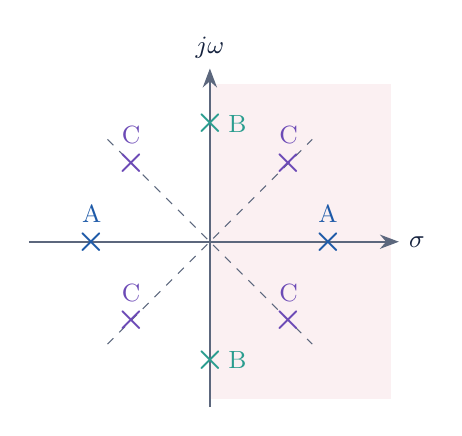
\begin{tikzpicture}[scale=1.0]
  \fill[ctrlcoral!8] (0,-2) rectangle (2.3,2);
  \draw[->,thick,ctrlgris] (-2.3,0) -- (2.4,0) node[right,text=ctrlnoche] {$\sigma$};
  \draw[->,thick,ctrlgris] (0,-2.1) -- (0,2.2) node[above,text=ctrlnoche] {$j\omega$};
  \draw[dashed,ctrlgris] (-1.3,-1.3) -- (1.3,1.3);
  \draw[dashed,ctrlgris] (-1.3,1.3) -- (1.3,-1.3);
  \foreach \x in {-1.5,1.5} {\node[text=ctrlazul,font=\large] at (\x,0) {$\boldsymbol\times$}; \node[text=ctrlazul,font=\small] at (\x,0.35) {A};}
  \foreach \y in {-1.5,1.5} {\node[text=ctrlverde,font=\large] at (0,\y) {$\boldsymbol\times$}; \node[text=ctrlverde,font=\small] at (0.35,\y) {B};}
  \foreach \x/\y in {-1/1,1/1,-1/-1,1/-1} {\node[text=ctrlvioleta,font=\large] at (\x,\y) {$\boldsymbol\times$}; \node[text=ctrlvioleta,font=\small] at (\x,\y+0.35) {C};}
\end{tikzpicture}
\end{document}
